\fancyfoot[C]{G�rel}
\subsection{Grundlagen ROS}
Das Robot Operating System (ROS) bietet ein flexibles und leistungsstarkes Ger�st f�r die Entwicklung von Software f�r Roboter und andere automatisierte Maschinen oder Anlagen. Es bietet eine Vielzahl von Werkzeugen, Bibliotheken und Konventionen, die Entwicklern dabei helfen, komplexe Anwendungen zu erstellen.

\paragraph{Modularit�t und Wiederverwendbarkeit: }
ROS ist auf Modularit�t ausgelegt, was bedeutet, dass verschiedene Komponenten eines Projekts als unabh�ngige Pakete entwickelt und wiederverwendet werden k�nnen. Dies erm�glicht eine saubere und strukturierte Entwicklung und erleichtert die Wartung und Skalierung von Systemen.

\paragraph{Kommunikation und Nachrichtenaustausch: }
Ein zentrales Konzept in ROS ist die Nachrichtenvermittlung, die es erm�glicht, dass verschiedene Teile eines Robotersystems miteinander kommunizieren k�nnen. ROS verwendet ein Publisher/Subscriber-Modell, bei dem Knoten Nachrichten �ber definierte Themen austauschen k�nnen. Dies erm�glicht eine lose Kopplung zwischen den Komponenten und erleichtert die Integration neuer Funktionen.

\paragraph{Publisher/Subscriber-Modell: }
ROS basiert auf einem Publisher/Subscriber-Modell, bei dem Knoten Nachrichten �ber definierte Themen austauschen k�nnen. Ein Knoten kann Nachrichten auf einem Thema ver�ffentlichen (\textit{publish}), und andere Knoten k�nnen sich auf dieses Thema abonnieren (\textit{subscribe}), um die Nachrichten zu empfangen. Dies erm�glicht eine lose Kopplung zwischen den Komponenten und erleichtert die Integration neuer Funktionen.
\begin{figure}[H]
    \centering
    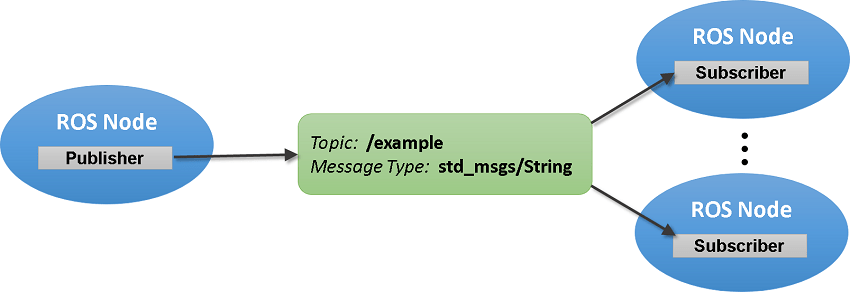
\includegraphics[scale=0.4]{./3_Stand_der_Technik/Abbildungen/ExchangeDataWithROSPublishersAndSubscribersExample_01.png}
    \caption{Illustration vom Nachrichtenaustausch der Nodes \cite{TheMathWorks2024}}
\end{figure}
\paragraph{Vordefinierte Nachrichtentypen: }
ROS bietet eine Vielzahl von vordefinierten Nachrichtentypen, die h�ufig in der Robotik verwendet werden. Dazu geh�ren Nachrichten wie \textit{LaserScan}, die Informationen �ber Laserabtastungen enthalten, oder \textit{IMU} (Inertial Measurement Unit), die Daten �ber die Orientierung und Bewegung eines Roboters liefern. Diese vordefinierten Nachrichtentypen erm�glichen eine einfache und standardisierte Kommunikation zwischen den verschiedenen Komponenten eines Robotersystems.

\paragraph{Anpassbare Nachrichten: }
Zus�tzlich zu den vordefinierten Nachrichtentypen k�nnen Entwickler auch eigene Nachrichtentypen definieren, um spezifische Anforderungen ihrer Anwendung zu erf�llen. Dies erm�glicht eine hohe Flexibilit�t und Anpassbarkeit bei der Entwicklung von Anwendungen und er�ffnet M�glichkeiten f�r die Integration neuer Sensoren, Aktuatoren und Algorithmen.
